




%\subsection{Description of the model}
The 2HDM+a model is a two Higgs doublet model with two scalar doublets $H_1$ and $H_2$ and an additional pseudoscalar singlet $P$. It is the simplest renormalizable extension of the simplified pseudoscalar mediator model with SM singlet Dark Matter, which makes the gauge symmetry manifest by coupling to the DM (here a Dirac fermion $\chi$) with the singlet $P$
%
\begin{equation} \label{eq:Lx}
{\cal L}_\chi = - i \hspace{0.25mm} y_\chi P \hspace{0.25mm} \bar \chi \hspace{0.25mm} \gamma_5 \hspace{0.1mm} \chi \,,
\end{equation}
while the Higgs doublets couple to the SM fermions 
\begin{equation} \label{eq:LY}
{\cal L}_{Y} = - \sum_{i=1,2} \left ( \bar Q Y_u^i \tilde H_i u_R  + \bar Q Y_d^i H_i d_R   + \bar L Y_\ell^i H_i \ell_R  + {\rm h.c.}  \right ) \,.
\end{equation}
The dominant mediator of interactions between the dark sector and the SM fermions is a superposition of the CP-odd component of $H_1$, $H_2$ and $P$. 
We impose a $Z_2$ symmetry under which $H_1\to H_1$ and $H_2\to -H_2$, such that only one Higgs doublet appears in each operator in \eqref{eq:LY}. The different ways to construct these operators result in different Yukawa coupling structures and we will remain as general as possible regarding this choice. 
The $Z_2$ symmetry is the minimal condition necessary to guarantee the absence of flavour-changing neutral currents (FCNCs) at tree-level \cite{Glashow:1976nt,Paschos:1976ay} and such a symmetry is realized in many well-motivated complete ultraviolet theories in the form of supersymmetry, a $U(1)$ symmetry or  a discrete symmetry acting on the Higgs doublets. We further choose all parameters in the scalar potential real, such that CP eigenstates are identified with the mass eigenstates, two scalars $h$ and $H$, two pseudoscalars $a$ and $A$, and a charged scalar $H^\pm$. Under these conditions, the most general scalar potential can be written as 
\begin{align}
V(P,H)=V_H+V_{PH}+V_P\,,
\end{align}
with the potential for the two Higgs doublets
\begin{align}\label{eq:VH}
V_{H} & = \mu_1 H_1^\dagger H_1 + \mu_2 H_2^\dagger H_2 + \left ( \mu_3  H_1^\dagger H_2 + {\rm h.c.} \right ) + \lambda_1  \hspace{0.25mm} \big ( H_1^\dagger H_1  \big )^2  + \lambda_2  \hspace{0.25mm} \big ( H_2^\dagger H_2 \big  )^2 \notag \\
& \phantom{xx} +  \lambda_3 \hspace{0.25mm} \big ( H_1^\dagger H_1  \big ) \big ( H_2^\dagger H_2  \big ) + \lambda_4  \hspace{0.25mm} \big ( H_1^\dagger H_2  \big ) \big ( H_2^\dagger H_1  \big ) + \left [ \lambda_5   \hspace{0.25mm} \big ( H_1^\dagger H_2 \big )^2 + {\rm h.c.} \right ]  \,,
\end{align}
potential terms which connect doublets and singlets 
\begin{equation} \label{eq:VHP}
\begin{split}
V_{HP}  = P \left ( i \hspace{0.1mm} b_P  \hspace{0.1mm}  H_1^\dagger H_2 + {\rm h.c.} \right ) + P^2 \left (  \lambda_{P1}  \hspace{0.1mm}  H_1^\dagger H_1 +   \lambda_{P2}  \hspace{0.1mm}  H_2^\dagger H_2 \right )  \,,
\end{split} 
\end{equation}
and the singlet potential
\begin{equation} \label{eq:VP}
V_{P}  =  \frac{1}{2} \hspace{0.5mm} m_P^2  P^2 +  \lambda_P\,P^4 \,.
\end{equation}
Upon rotation to the mass eigenbasis, we trade the five dimensionful and eight dimensionless parameters in the potential  for physical masses and mixing angles and three quartic couplings
\begin{align}
\left\{ \,\,\begin{matrix}
\mu_1,\,\mu_2,\\[3pt]
\mu_3\,, m_P^2,\, b_P\\[3pt]
\lambda_1\,,\lambda_2\,,\lambda_3\,,\lambda_4\,,\lambda_5\\
\lambda_{P1}\,,\lambda_{P2} \,, \lambda_P
\end{matrix}\,\,\right\}\qquad \quad \longleftrightarrow \quad \qquad \left\{ \,\,\begin{matrix}
v,\, M_h,\,\cos(\beta-\alpha)\\[3pt]
M_a\,, M_A\,, M_H\,,M_{H^\pm}\\[3pt]
t_\beta\,, \cos(\theta)\,, \\[3pt]
\lambda_3\,,\lambda_{P1}\,,\lambda_{P_2}\,,\lambda_P
\end{matrix}\,\,\right\}\,.
\end{align}
Out of these parameters, the electroweak scale $v=246$ GeV and the mass of the SM-like CP-even mass eigenstate $M_h=125$ GeV are fixed. The mixing angle $\alpha$ between the CP-even scalars $h$ and $H$ is constrained by Higgs coupling strength measurements \cite{} and we show the allowed parameter space in the $\cos(\beta-\alpha)$ plane in  Fig.~\ref{fig:higgsfit} for the Yukawa sector of a 2HDM of type II.  For arbitrary values of $t_\beta=v_2/v_1$ only the limit $\cos(\beta-\alpha)\approx 0$ is allowed, for which the couplings of the CP-even state $h$ align with the couplings of the SM Higgs boson. For the analyses discussed in the remainder of this paper, we choose this so-called alignment limit and treat $t_\beta$ as a free parameter.
%%
\begin{figure}[t]
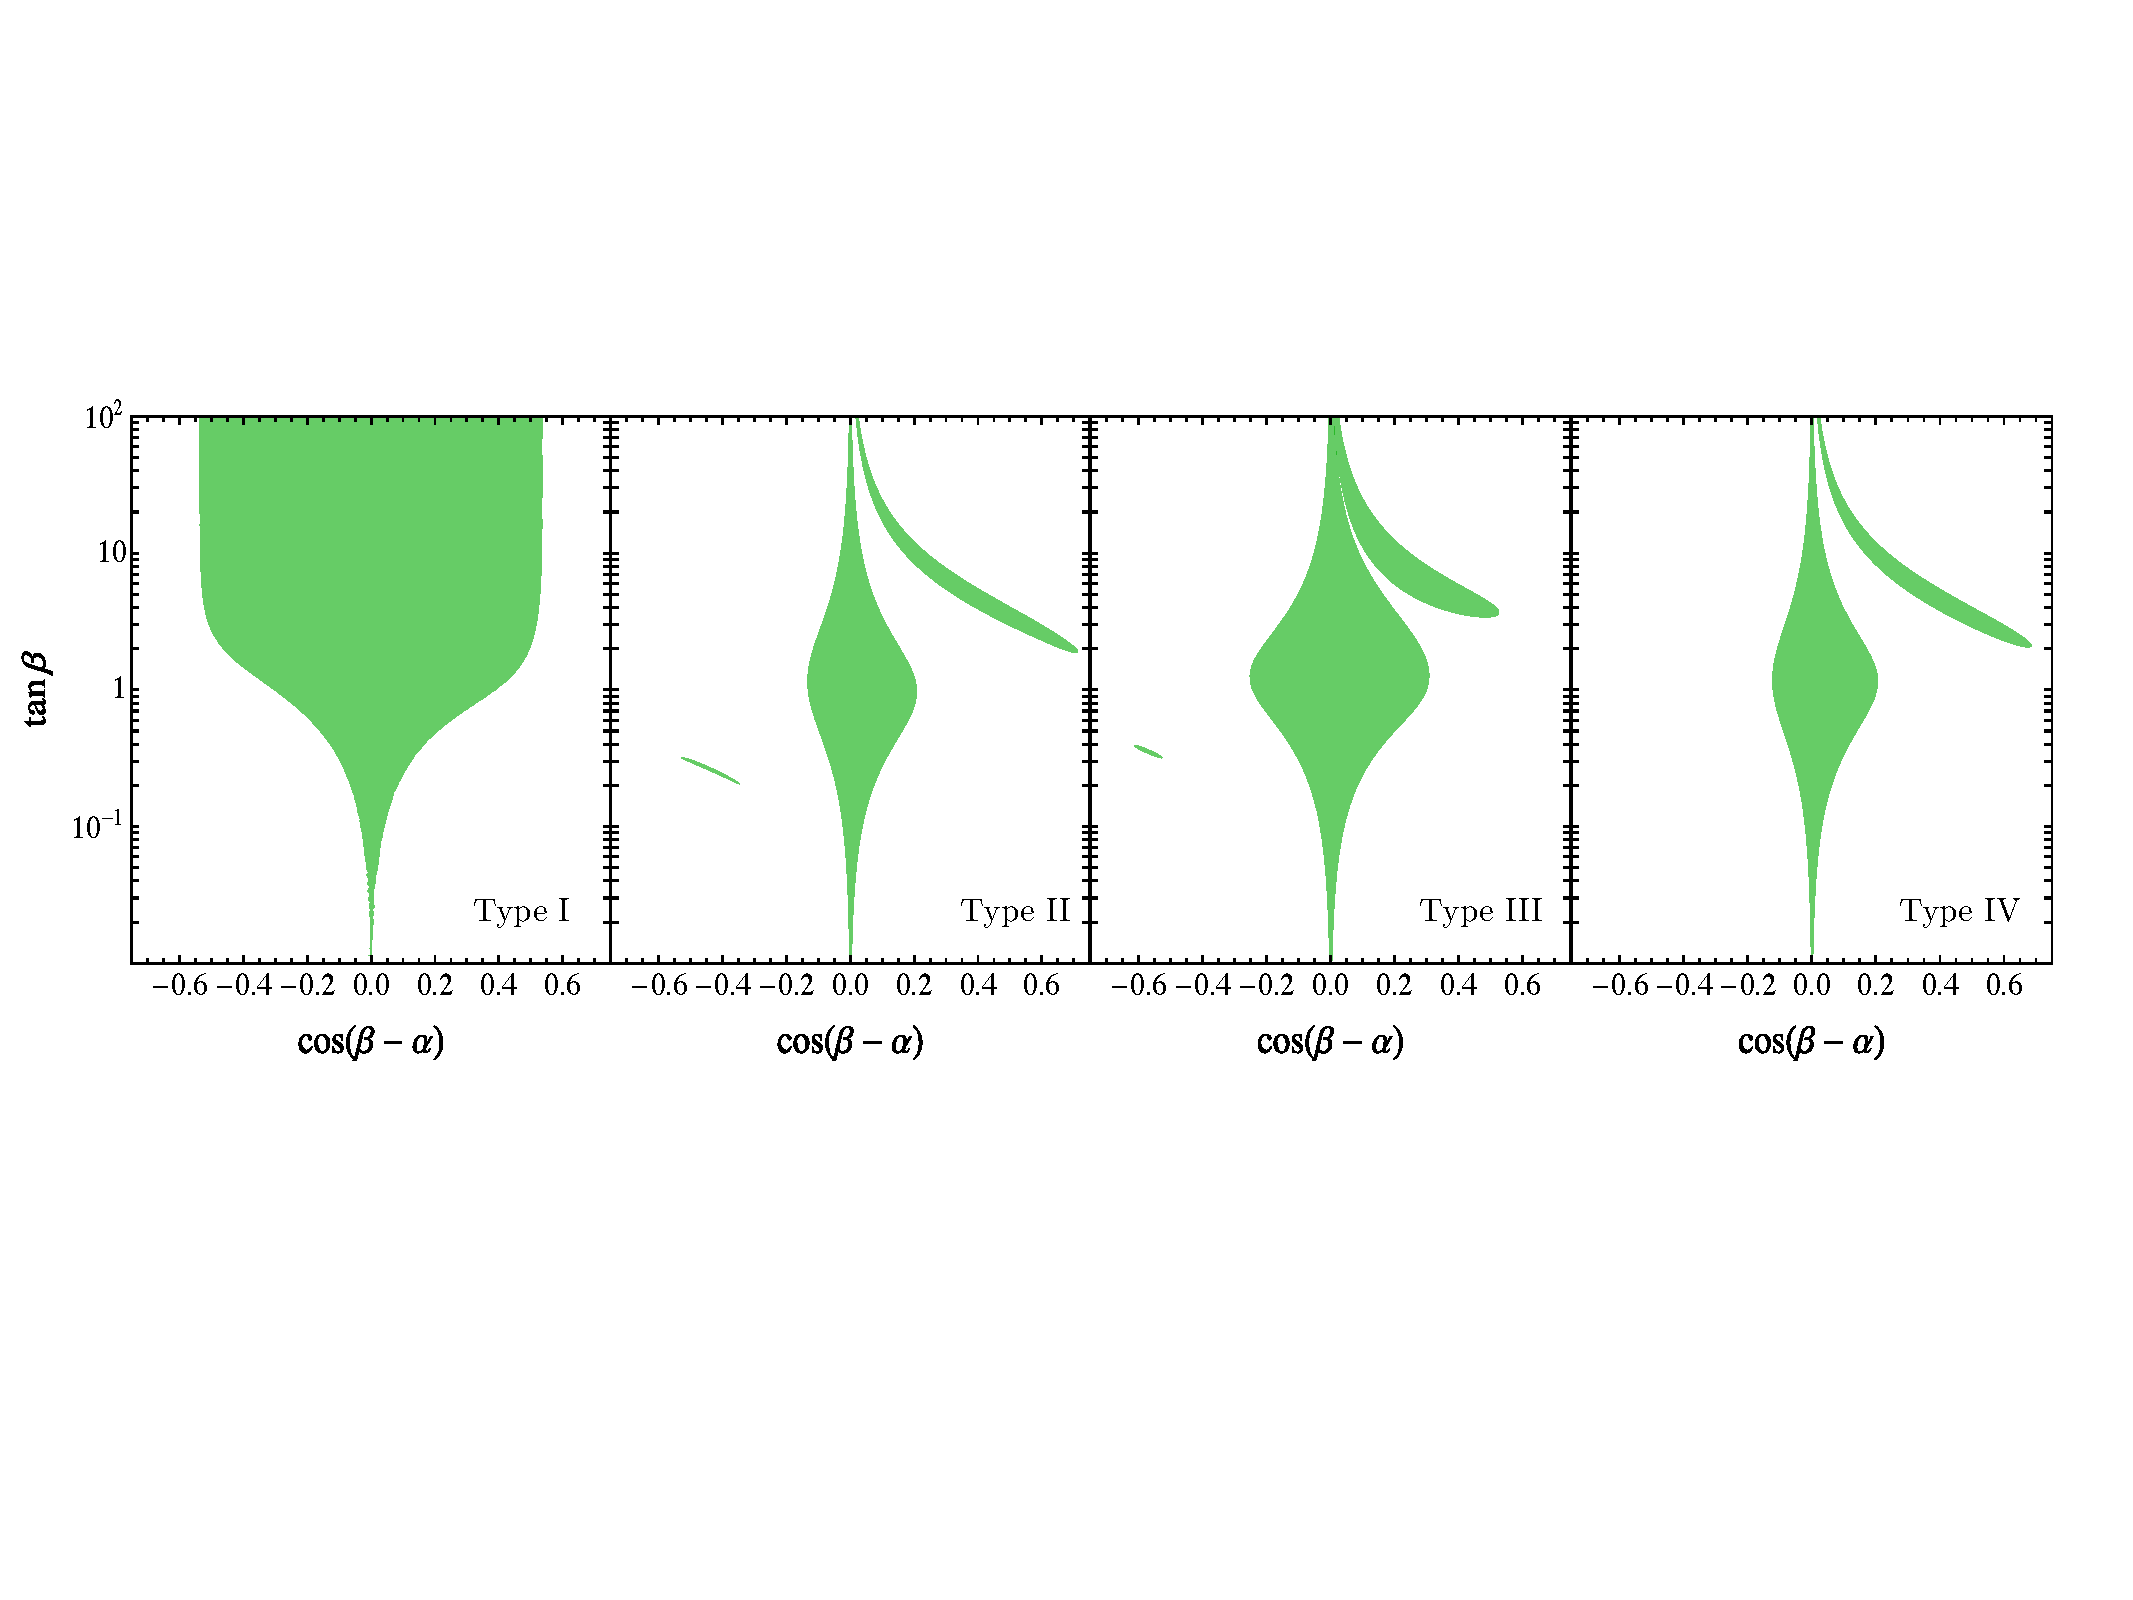
\includegraphics[width=\textwidth]{texinputs/03_theoparameters/Figs/Higgsfit}
\caption{\label{fig:higgsfit} Parameter space allowed by a global fit to Higgs coupling strength measurements for (from left to right) a Yukawa sector of type I ($Y_u^1  = Y_d^1 = Y_\ell^1 =0$), type II ($Y_u^1 = Y_d^2 = Y_\ell^2 =0$),  type III ($Y_u^1 = Y_d^1 = Y_\ell^2 =0$), and type IV ($Y_u^1  = Y_d^2 = Y_\ell^1 =0$). }
\end{figure}
%%
Electroweak precision measurements constrain the splitting between the masses $M_H, M_A, M_a$ and $M_{H^\pm}$, since loops of spin-0 states modify the propagators of the electroweak gauge bosons at one-loop. For $M_H=M_{H^\pm}$ and $\cos(\beta-\alpha)=0$, these corrections vanish due to a custodial symmetry in the tree-level potential $V_H$ \cite{} and the masses of the CP-odd mass eigenstates can be treated as free parameters. This custodial symmetry is also present in $V_H$ if $M_A=M_{H^\pm}$ and $\cos(\beta-\alpha)=0$, but the presence of the pseudoscalar mixing term in $V_P$ softly breaks this symmetry. As a consequence, the pseudoscalar mixing angle $\theta$ and the mass splitting between $M_H$, $M_A$ and $M_a$ are constrained in this situation. In Fig.~\ref{fig: EWPTs}...
Flavour observables are mostly sensitive to corrections from one-loop exchanges of the charged scalar ${H^\pm}$, whose contributions to $b \to X_s \gamma$ \cite{Hermann:2012fc,Misiak:2015xwa,Czakon:2015exa} and $B_s-\bar B_s$ mixing \cite{Abbott:1979dt,Geng:1988bq,Buras:1989ui,Eberhardt:2013uba} lead to the strongest indirect constraints on $M_{H^\pm}$. Since the couplings of the charged scalar only depend on $t_\beta$, these constraints result in the bound $\tan \beta \gtrsim 0.8$ for $M_{H^\pm}=750$ GeV, independent of the choice of the Yukawa sector.\\
%%
\begin{figure}
\centering
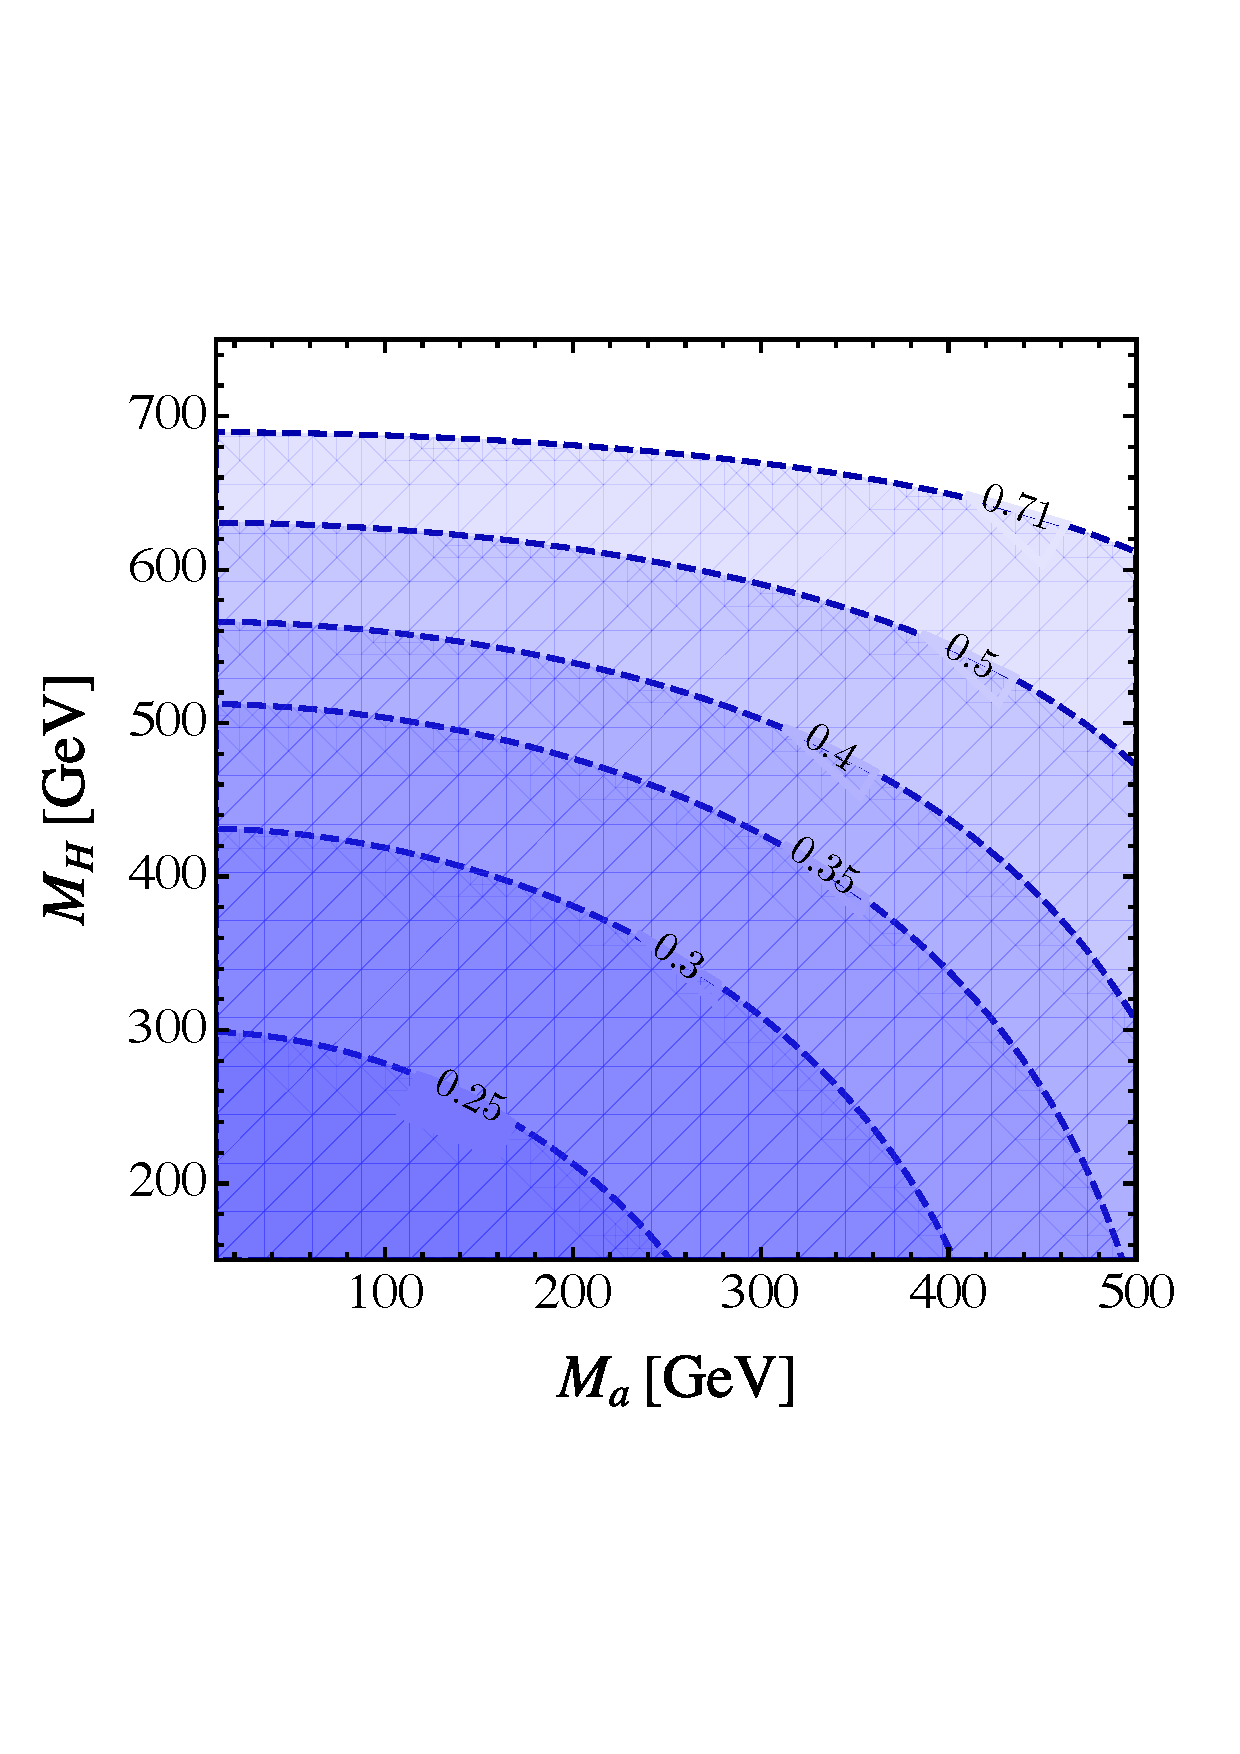
\includegraphics[width=.5\textwidth]{texinputs/03_theoparameters/Figs/EWPM}
\caption{\label{fig:EWPM}Values of $M_H$ and $M_a$ allowed by electroweak precision constraints for $\cos(\beta-\alpha)=0, M_{H^\pm}=M_A=750$ GeV, and varying values of the pseudoscalar mixing angle $\sin \theta =0.25, 0.3, 0.35, 0.4, 0.5$ , and maximal mixing angle $\sin\theta =1/\sqrt{2}\approx 0.71$. The parameter space below and to the left of the dashed contours is excluded. }
\end{figure}
%%
In addition to these constraints, the potential $V_H$ needs to give rise to a stable vacuum breaking the electroweak symmetry, whereas the parameters in $V_P$ need not introduce a vacuum expectation value for $P$, and scattering amplitudes should remain perturbative \cite{Gunion:2002zf,Barroso:2013awa} and unitary \cite{Kanemura:1993hm,Akeroyd:2000wc,Ginzburg:2005dt,Grinstein:2015rtl} up to the UV scale, where the 2HDM+a is UV completed by a more complete theory.  These conditions impose additional constraints on the quartic couplings in the potential, which are satisfied for $M_H, M_A, M_a \lesssim \mathcal{O}(1)$ TeV and $\lambda_3, \lambda_{P1}, \lambda_{P2}$ and $\lambda_P$ of $\mathcal{O}(1)$ as long as $t_\beta$ is not too much smaller than one. For the case of fixed\footnote{The singlet quartic $\lambda_P$ is entirely irrelevant for the phenomenology of the 2HDM+a.} $\lambda_3, \lambda_{P1}, \lambda_{P2}$, the stability condition therefore leads to additional constraints on the mixing angle $\theta$ and the masses. The parameter space of the 2HDM+a is strongly constrained, as summarized below
%
\newline
\begin{tabular}{cc c}
&&\\
$v, M_h, \cos(\beta-\alpha) $&$\longleftrightarrow$& fixed by Higgs measurements,\\[.3cm]
$M_{H^\pm}\,, $  &$\longleftrightarrow $& constrained by flavour observables,\\[.3cm]
$\sin(\theta)\,, M_H \,\,\text{or} \,\,M_A$  &$\longleftrightarrow $& constrained EWPM,\\[.3cm]
$\lambda_3, \lambda_{P1}, \lambda_{P2}\,,\lambda_P $ &$\longleftrightarrow $& constrained by stability, perturbativity and unitarity constraints\,.\\[.3cm]
&&
\end{tabular}
\newline
%
This leaves us with effectively three three free parameters from the potential, the Dark Matter mass and the coupling of the mediator to the DM candidate
\begin{align}
\big\{ m_\chi\,,\,\,M_a\,,\,\, t_\beta\,, \,\, M_H\,\,\text{or}\,\,M_A\,\,, \,\, y_\chi\,\big\}\,.
\end{align}
%In comparison,  the simplified model with a singlet mediator can be described with four parameters: the dark matter mass $m_{DM}$, the mass of the mediator $m_a$, the interaction strength between the mediator and the SM fermions $g_q$, and between the mediator and the DM candidate $g_\text{DM}$.

%\begin{thebibliography}{999}
%
%%\cite{Beltran:2010ww}
%\bibitem{Beltran:2010ww} 
%M.~Beltran, D.~Hooper, E.~W.~Kolb, Z.~A.~C.~Krusberg and T.~M.~P.~Tait,
%%``Maverick dark matter at colliders,''
%JHEP {\bf 1009}, 037 (2010)
%%  doi:10.1007/JHEP09(2010)037
%[arXiv:1002.4137 [hep-ph]].
%%%CITATION = doi:10.1007/JHEP09(2010)037;%%
%%286 citations counted in INSPIRE as of 25 Feb 2018
%
%%\cite{Fox:2011pm}
%\bibitem{Fox:2011pm} 
%P.~J.~Fox, R.~Harnik, J.~Kopp and Y.~Tsai,
%%``Missing Energy Signatures of Dark Matter at the LHC,''
%Phys.\ Rev.\ D {\bf 85}, 056011 (2012)
%doi:10.1103/PhysRevD.85.056011
%[arXiv:1109.4398 [hep-ph]].
%%%CITATION = doi:10.1103/PhysRevD.85.056011;%%
%%408 citations counted in INSPIRE as of 25 Feb 2018
%
%%\cite{Goodman:2010ku}
%\bibitem{Goodman:2010ku} 
%J.~Goodman, M.~Ibe, A.~Rajaraman, W.~Shepherd, T.~M.~P.~Tait and H.~B.~Yu,
%%``Constraints on Dark Matter from Colliders,''
%Phys.\ Rev.\ D {\bf 82}, 116010 (2010)
%%  doi:10.1103/PhysRevD.82.116010
%[arXiv:1008.1783 [hep-ph]].
%%%CITATION = doi:10.1103/PhysRevD.82.116010;%%
%%544 citations counted in INSPIRE as of 25 Feb 2018
%
%
%\end{thebibliography}

\begin{itemize}
    \item Motivate the choice of parameters in~\cite{Bauer:2017ota}
    
    
    \item Vacuum stability study: fix lambda parameters to 3
    
    For extension of the Higgs sector (and in general for scalar extensions of the Standard Model) one needs to worry about 
    boundedness from below of the scalar potential, as well as absolute stability of the electroweak minimum\footnote{We remark 
    here that implications from all indirect constraints - be it flavour, electroweak precision constraints or stability 
    requirements -  should be treated as preferred parameter space in a simplified model framework. It would contradict the idea of simplified
models were these constraints taken at face value.}.  

    Regarding boundedness from below of the scalar potential in the present 2HDM + S model, we stress that provided that 
    $\lambda_{P1}, \, \lambda_{P2} > 0$ in
    %
    \begin{eqnarray}
     V_{\mathrm{P}} = \frac{1}{2} m_{P}^2 P^2 + \kappa\, (i \,P\, H_1^{\dagger}H_2 + \mathrm{h.c.}) \nonumber \\
            + \lambda_{P1} \,P^2\, \left|H_1\right|^2 + \lambda_{P2} \,P^2 \,\left|H_2\right|^2 \, ,\nonumber
    \end{eqnarray}
    %
    the study of boundedness from below at tree-level reduces to the corresponding study in the 2HDM. The boundedness from below conditions 
    in this case are well-known~\cite{Gunion:2002zf}:
    %
    \begin{equation}
    \label{stability2HDM}
     \lambda_1 > 0\,, \,\,\, \lambda_2 > 0\,, \,\,\, \lambda_3 > - \sqrt{\lambda_1 \lambda_2} \,, \,\,\, \lambda_3 + \lambda_4 - |\lambda_5| > - \sqrt{\lambda_1 \lambda_2} 
    \end{equation}
    %
    and can be inferred from analyzing the scalar potential at large field values $H_1,\,H_2 \gg v$. For $m_{H^{\pm}} = m_{H_0}$, the first two conditions 
    in~\eqref{stability2HDM} may be simply written as
    %
    \begin{equation}
     \frac{m_h^2}{v^2} (1-t_{\beta}^{2}) + \lambda_3 \, t_{\beta}^{2} > 0\,, \quad\,\, \frac{m_h^2}{v^2} (1-t_{\beta}^{-2}) + \lambda_3 \, t_{\beta}^{-2} > 0
     \end{equation}
    %
    which result in the requirement $\lambda_3 > m_h^2/v^2 = 0.258$. In figure~\ref{Fig_Stability} we show the regions of parameter space in the 
    ($m_a,\, m_{H_0}$) (left) and ($s_{\theta},\, m_a$) (right) planes for which the tree-level boundedness from below conditions~\ref{stability2HDM}
    are satisfied, assuming $m_{H^{\pm}} = m_{H_0} = m_{A_0}$.
    %
    %
    \begin{figure}[h!]
\begin{center}
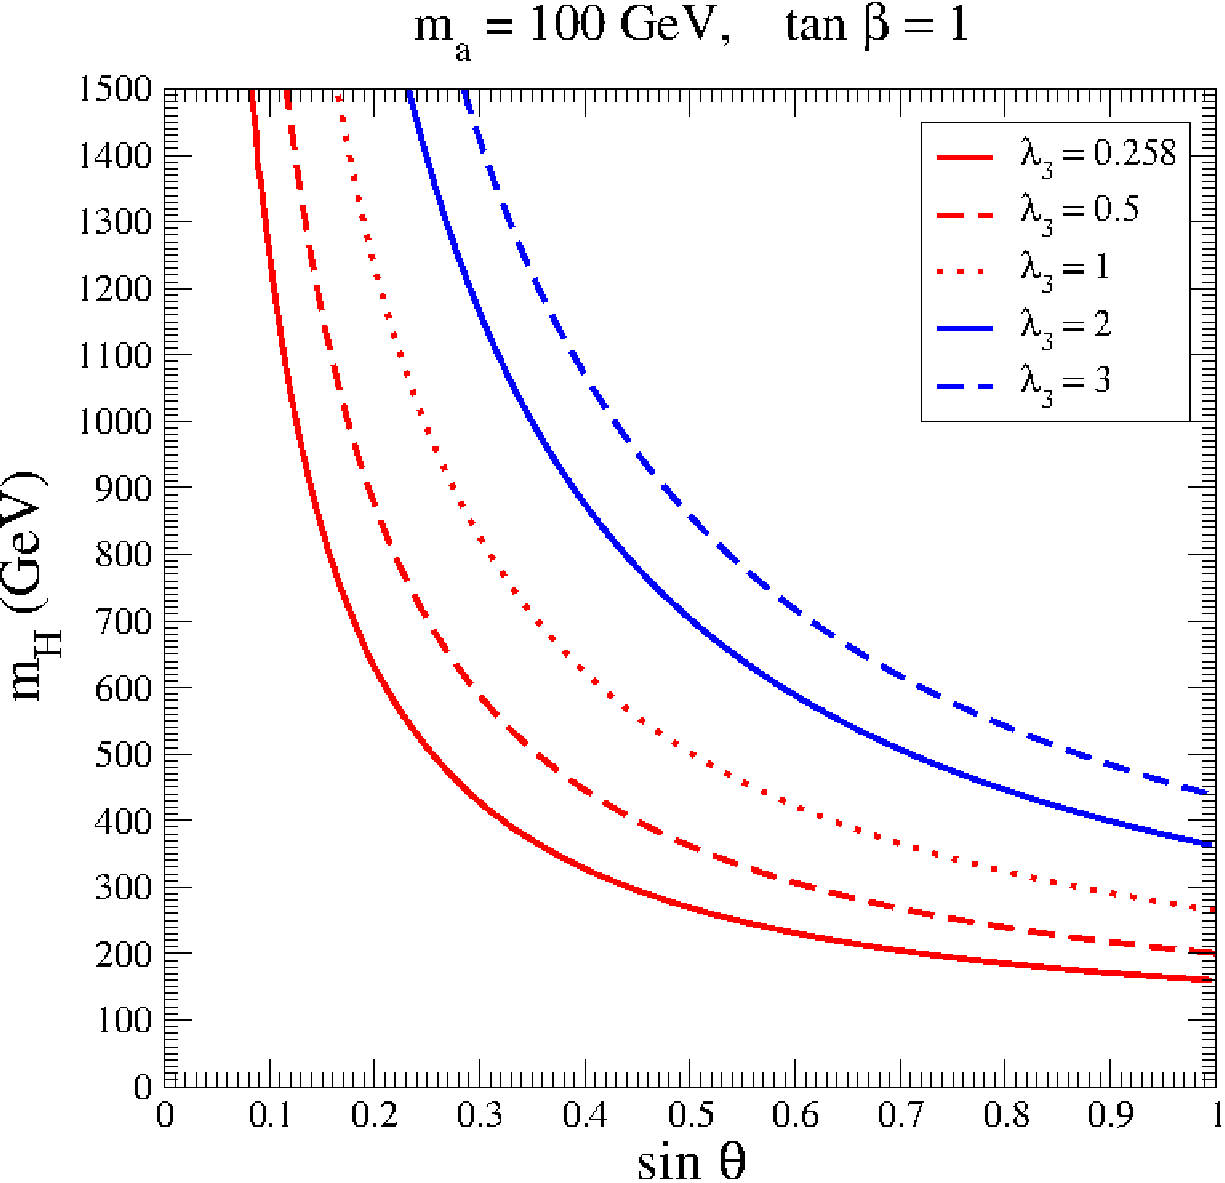
\includegraphics[width=0.485\textwidth]{texinputs/03_theoparameters/Figs/Plot_Eq.pdf}
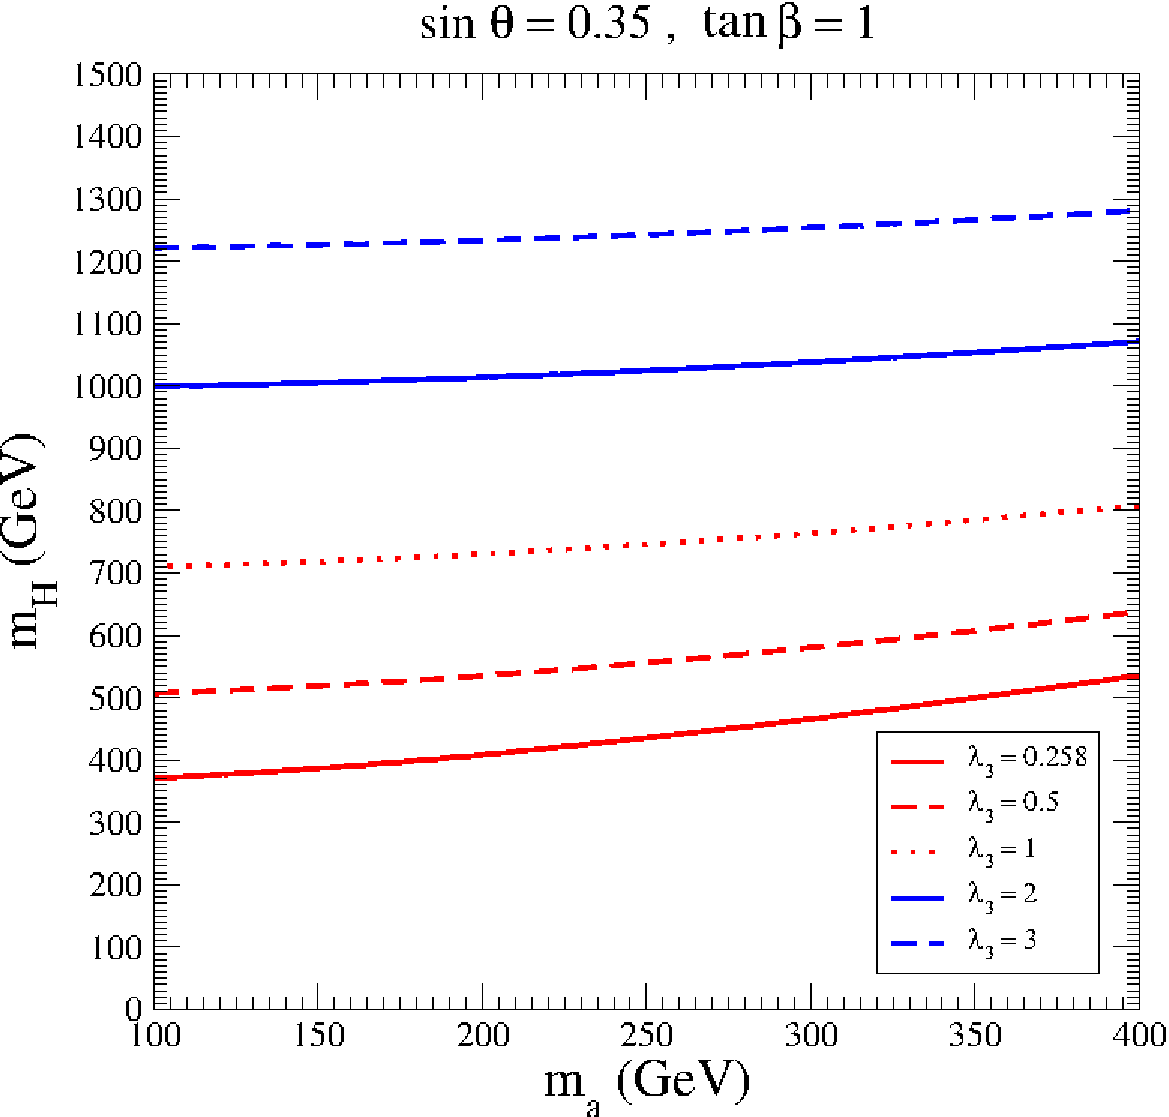
\includegraphics[width=0.485\textwidth]{texinputs/03_theoparameters/Figs/Plot_ma.pdf}
\caption{\small Regions of parameter space in the 
    ($m_a,\, m_{H_0}$) (left) and ($s_{\theta},\, m_a$) (right) planes for which the tree-level boundedness from below conditions~\ref{stability2HDM}
    are satisfied, assuming $m_{H^{\pm}} = m_{H_0} = m_{A_0}$. 
}
\label{Fig_Stability}
\end{center}

\vspace{-2mm}

\end{figure}
    %
    %
    
    Figure~\ref{Fig_Stability} shows that the region satisfying the tree-level boundedness from below conditions increases as $\lambda_3$ increases. At the same time, 
    the choice $\lambda_3 = \lambda_{P1} = \lambda_{P2}$ which we adopt in the present analysis allows the increase in $\lambda_3$  not to affect the mono-Higgs sensitivity
    via a change in the coupling $g_{aAh}$
    %
    \begin{eqnarray}
     g_{aAh} &=& \frac{c_{\theta} \,s_{\theta}}{m_{H} \,v} \left[m_h^2 + m_H^2 -m_a^2 - 2 
     (\lambda_3 - \lambda_{P1} c_{\beta}^2 - \lambda_{P2} s_{\beta}^2) v^2 \right] \nonumber \\
      &=& \frac{c_{\theta} \,s_{\theta}}{m_{H} \,v} \left[m_h^2 + m_H^2 -m_a^2 \right] 
    \end{eqnarray}
    %
    We then fix the value $\lambda_3 = 3$ as benchmark for the rest of our analysis. 
    
    \vspace{3mm}
    
    A few comments are in order. 
    
    \begin{itemize}
     \item The choice of $\lambda_3$, motivated by boundedness from below conditions, while not affecting the mono-Higgs sensitivity 
    if $\lambda_3 = \lambda_{P1} = \lambda_{P2}$, has an impact on the mono-$Z$ sensitivity since the coupling 
    %
    \begin{eqnarray}
     g_{Haa} &=& \frac{1}{m_{H} \,v} \left[ 2\, t_{2\beta}^{-1}\, s_{\theta}^2\, 
(m_h^2 - \lambda_3 v^2) + s_{2\beta}\, c_{\theta}^2 v^2 (\lambda_{P1} - \lambda_{P2}) \right] \nonumber \\
      &=& \frac{1}{m_{H} \,v} \left[ 2\, t_{2\beta}^{-1}\, s_{\theta}^2\, 
(m_h^2 - \lambda_3 v^2) \right] 
    \end{eqnarray}
    %
    does depend on $\lambda_3$ and influences the balance between $\Gamma(H_0 \to aa)$ and $\Gamma(H_0 \to Za)$ which ultimately determines the 
    $H_0 \to Za$ branching fraction. In short, the choice of $\lambda_3$, $\lambda_{P1}$, $\lambda_{P2}$ affects either mono-Higgs or mono-$Z$ sensitivities
    (or both).
    
    \item Together with boundedness from below, other potential constraints are usually considered in the context of the 2HDM and apply in general, 
    among them unitarity (see e.g.~\cite{Ginzburg:2005dt,Grinstein:2015rtl}) and absolute stability of the electroweak vacuum (see e.g.~\cite{Barroso:2013awa}). 
    In the present context we find these constraints 
    are generically weaker than the boundedness from below condition and therefore disregard them in the following. 
    
    \item The boundedness from below conditions are here evaluated at tree-level, but in a fully consistent treatment 
    they should be evaluated including the effect of radiative corrections. This is however 
    a much more involved process than what has been discussed above for the 
    tree-level case (see e.g.~\cite{Staub:2017ktc}). In addition, 
    the boundedness from below constraints discussed here are potentially sensitive to the 
    existence of UV physics which our 2HDM+S simplified does not capture, and which could modify the above picture through the presence of higher-dimensional 
    operators. Still, it is worth pointing out that for the 2HDM+S simplified model to be a good description of LHC phenomenology we require 
    the new physics scale suppressing these effective operators to be above the TeV scale (since in our scans we are considering scalar masses up to $\sim 1$ TeV), 
    and thus the presence of these high-energy operators is not expected to be of much help in case a runaway field direction exist at tree level in the 2HDM scalar 
    potential.
    \end{itemize}
    
    
    
    
\end{itemize}


